\subsection{Proof Of Concept}\label{subsec:poc}

\subsubsection*{Überblick}

Um sicherzustellen, dass die Anforderungen an das System mit den gewählten Technologien umgesetzt werden
können, wird zunächst ein Proof Of Concept implementiert. Dieser Proof Of Concept hat einen deutlich kleineren
Funktionsumfang als das Endprodukt.

\subsubsection*{Funktionsumfang}

Im Wesentlichen muss der Proof Of Concept beweisen, dass es möglich ist mit den
gewählten Technologien Benachrichtigungen zu Versenden und zu Empfangen.



\begin{figure}[h]
    \centering
    \begin{minipage}[b]{1.0\textwidth}
        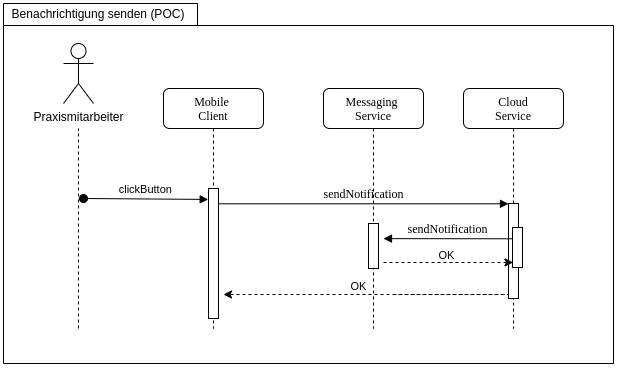
\includegraphics[width=\textwidth]{graphics/Sequence_POC_Send}
        \caption{Proof Of Concept - Benachrichtigung versenden}
    \end{minipage}
\end{figure}



blablabla




\begin{figure}[h]
    \centering
    \begin{minipage}[b]{1.0\textwidth}
        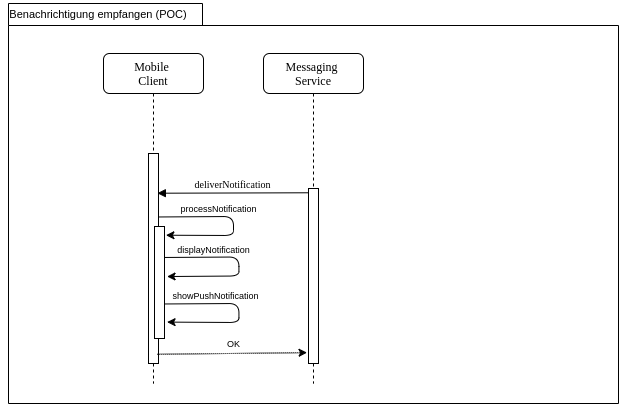
\includegraphics[width=\textwidth]{graphics/Sequence_POC_Receive}
        \caption{Proof Of Concept - Benachrichtigung empfangen}
    \end{minipage}
\end{figure}


blablala





\textbf{U01 - Benachrichtigungen versenden}

Mit dem Proof Of Concept muss es möglich sein, Benachrichtigungen von einem Client zu versenden.

Abgrenzung:
\begin{itemize}
    \item Der Sender hat einen Button um Benachrichtigungen zu versenden
    \item Das System ist nicht konfigurierbar
    \item Das System unterstützt keine Authentifikation
    \item
    \item Notifikation wird vom Client gesendet und vom selben Client empfangen.
    \item Keine Authentication oder Authorization.
\end{itemize}


\textbf{U02 - Benachrichtigungen empfangen}

Mit dem Proof Of Concept muss es möglich sein, Benachrichtigungen mit einem Client zu empfangen.


\textbf{T01 - IPad Client}

Der für den Proof Of Concept umgesetzte Client muss auf einem IPad funktionieren und alle Anforderungen die an den
Proof Of Concept gestellt werden erfüllen. Kommunikation mit Cloud Service muss funktionieren. Kommunikation mit Messaging Service muss funktionieren.


\textbf{T04 - AWS Platform}

Der Cloud Service muss auf AWS deployed werden. Die Kommunikation zwischen Mobile Client und Cloud Service muss funktionieren.
Die Kommunikation mit Messaging Service muss funktionieren.



\subsubsection*{Restriktionen}
\begin{itemize}
    \item Nur 1 Client.
    \item Nur 1 fixe Notifikation. Keine Types.
    \item Notifikation wird vom Client gesendet und vom selben Client empfangen.
    \item Keine Authentication oder Authorization.
\end{itemize}

\clearpage
